\section{Integraci�n Sem�ntica de una Memoria Corporativa}
%%%%%%%%%%%%%%%%%%%%%%%%%%%%%%%%%%%%%%%%%%%%%%%%%%%%%%%%%%%%%%%%%%%%%%%%%%%%%%
\subsection{Marco de Referencia}
\begin{frame}
	\frametitle{Marco de Referencia}
	\begin{block}{Etapas}
		\begin{enumerate}
		\item \justifying \textbf{\textit{Representaci�n del conocimiento explicito de los recursos}} consiste en identificar los recursos de informaci�n de la memoria corporativa, as� como representar las caracter�sticas y relaciones (conocimiento expl�cito) de estos recursos en un modelo sem�ntico.
		\item \justifying \textbf{\textit{Enriquecimiento del conocimiento en el modelo}} consiste en introducir reglas de inferencia (axiomas) para completar y enriquecer el modelo sem�ntico con conocimiento impl�cito del dominio de la memoria corporativa.
		\item \justifying \textbf{\textit{B�squeda y recuperaci�n de la informaci�n en el modelo}} consisten en identificar las principales consultas de los usuarios, as� como interrogar el modelo sem�ntico para recuperar la informaci�n que responda a estas consultas.
		\end{enumerate}
	\end{block}
\end{frame}
%%%%%%%%%%%%%%%%%%%%%%%%%%%%%%%%%%%%%%%%%%%%%%%%%%%%%%%%%%%%%%%%%%%%%%%%%%%%%%

%%%%%%%%%%%%%%%%%%%%%%%%%%%%%%%%%%%%%%%%%%%%%%%%%%%%%%%%%%%%%%%%%%%%%%%%%%%%%%
\subsection{Arquitectura de la Integraci�n Sem�ntica}
\begin{frame}
	\frametitle{Arquitectura de la Integraci�n Sem�ntica}	
	\begin{figure}
	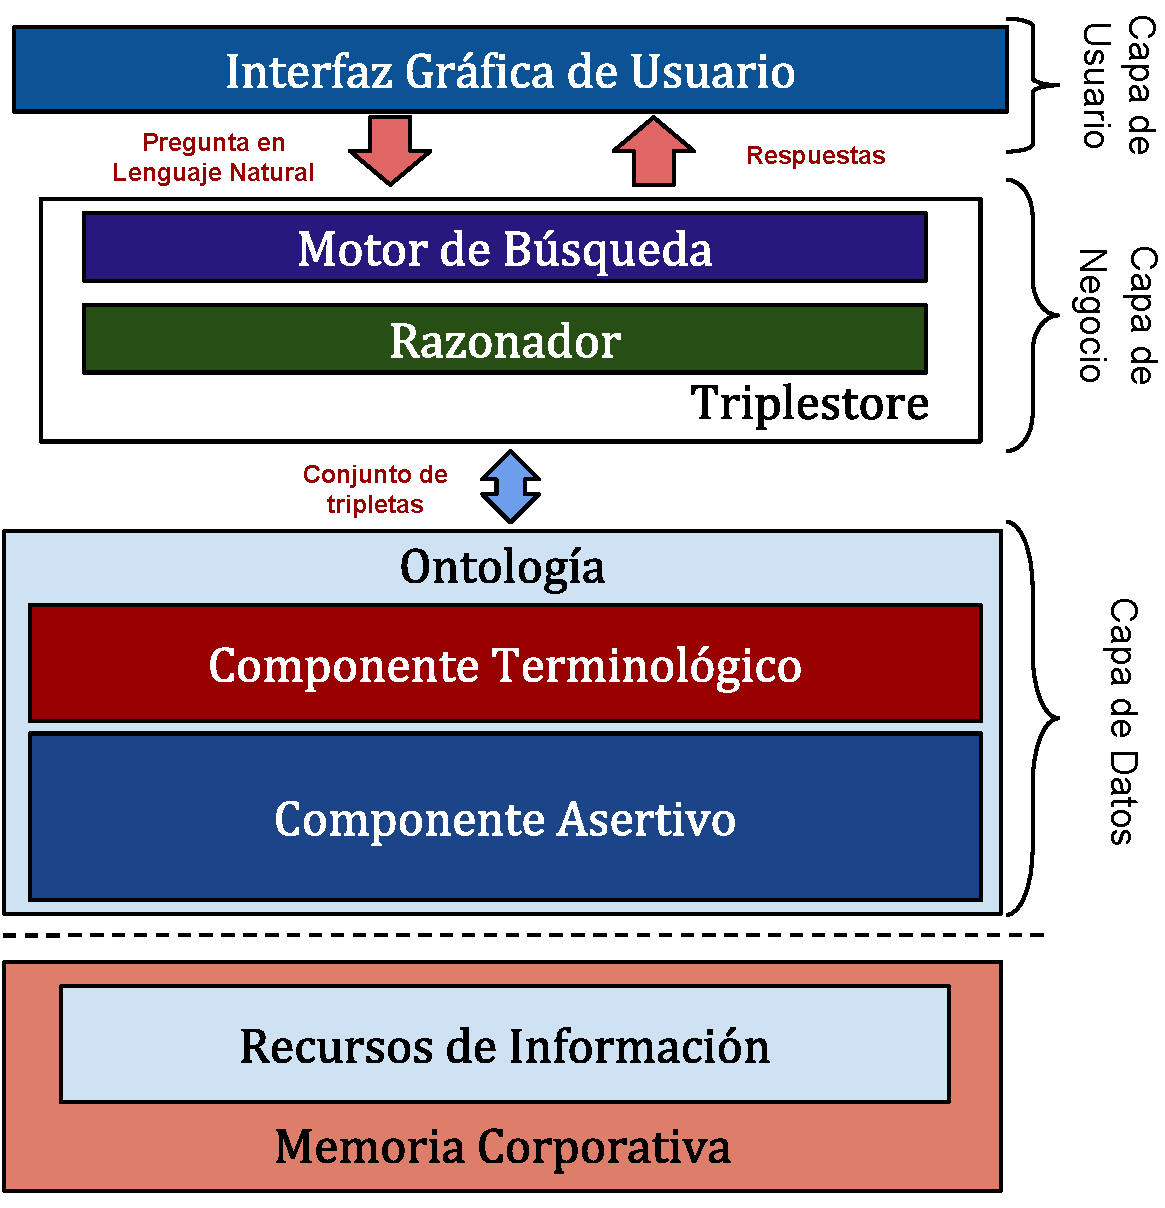
\includegraphics[scale=0.35]{Arquitectura} 
	\end{figure}
\end{frame}
%%%%%%%%%%%%%%%%%%%%%%%%%%%%%%%%%%%%%%%%%%%%%%%%%%%%%%%%%%%%%%%%%%%%%%%%%%%%%%

%%%%%%%%%%%%%%%%%%%%%%%%%%%%%%%%%%%%%%%%%%%%%%%%%%%%%%%%%%%%%%%%%%%%%%%%%%%%%%
\subsection{Casos de Uso}
\begin{frame}
	\frametitle{Casos de Uso}
	
	\begin{block}{}
		\begin{itemize}
		\item \justifying \textbf{\textit{Cartograf�a de Competencias}} consiste en la b�squeda y recuperaci�n de informaci�n significativa de las personas a partir de las caracter�sticas personales y profesionales de las mismas.
		\item \justifying \textbf{\textit{B�squeda de Recursos Digitales}} consiste en la b�squeda y recuperaci�n de informaci�n significativa de los documentos y archivos multimedia a partir del contenido de los mismos.
		\end{itemize}
	\end{block}
	
	\begin{figure}
	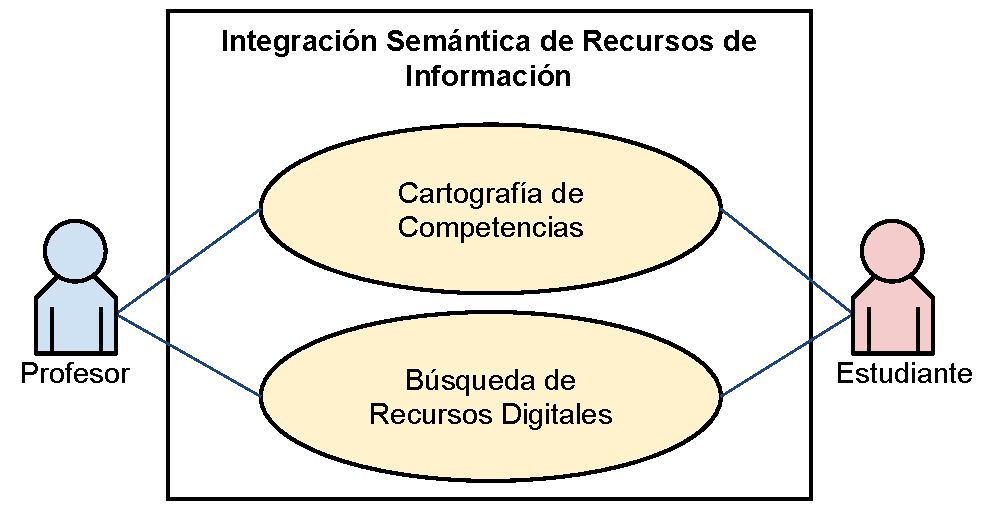
\includegraphics[scale=0.65]{CasosUso} 
	\end{figure}
\end{frame}
%%%%%%%%%%%%%%%%%%%%%%%%%%%%%%%%%%%%%%%%%%%%%%%%%%%%%%%%%%%%%%%%%%%%%%%%%%%%%%

%%%%%%%%%%%%%%%%%%%%%%%%%%%%%%%%%%%%%%%%%%%%%%%%%%%%%%%%%%%%%%%%%%%%%%%%%%%%%%
\subsection{Representaci�n el Conocimiento}
\subsubsection{Identificar los principales recursos de informaci�n}
\begin{frame}
	\frametitle{Identificar los principales recursos de informaci�n}	
	\begin{figure}
	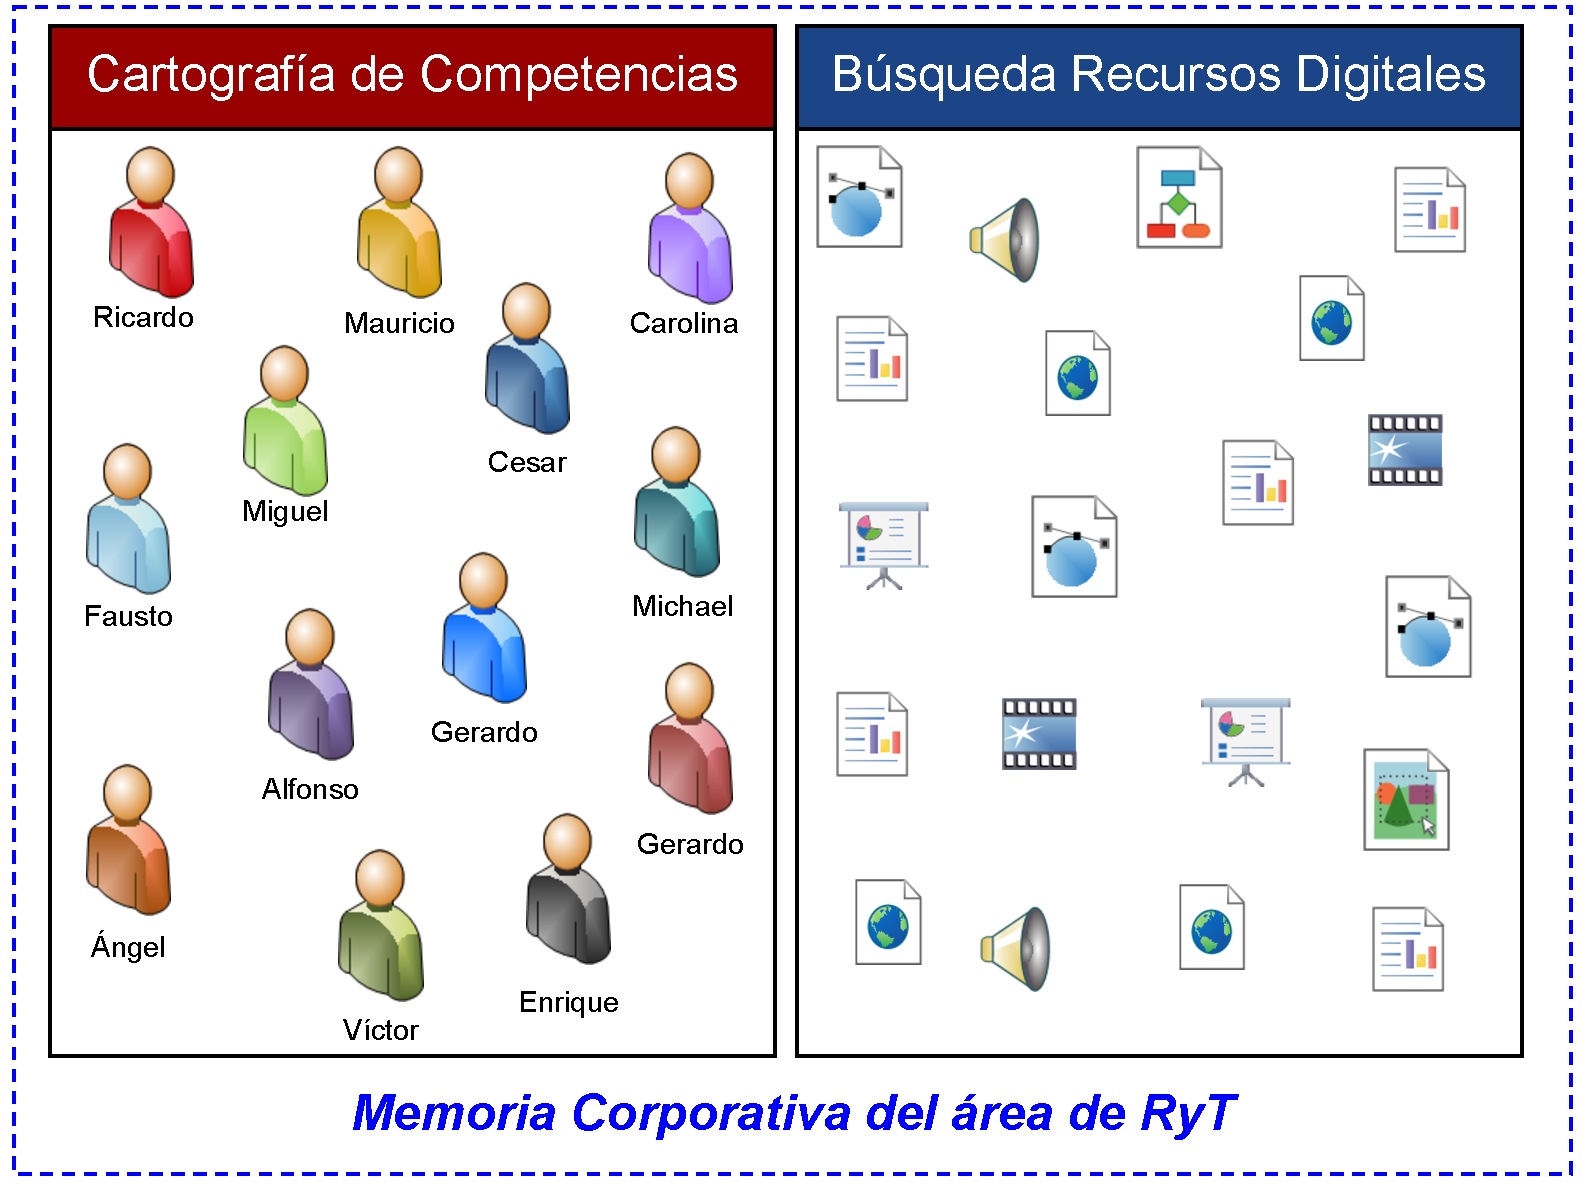
\includegraphics[scale=0.35]{CasosUsoMC} 
	\end{figure}
\end{frame}

\subsubsection{Adquirir y expresar el conocimiento de los recursos de informaci�n}
\begin{frame}
	\frametitle{Adquirir y expresar el conocimiento de los recursos de informaci�n}	
	\begin{figure}
	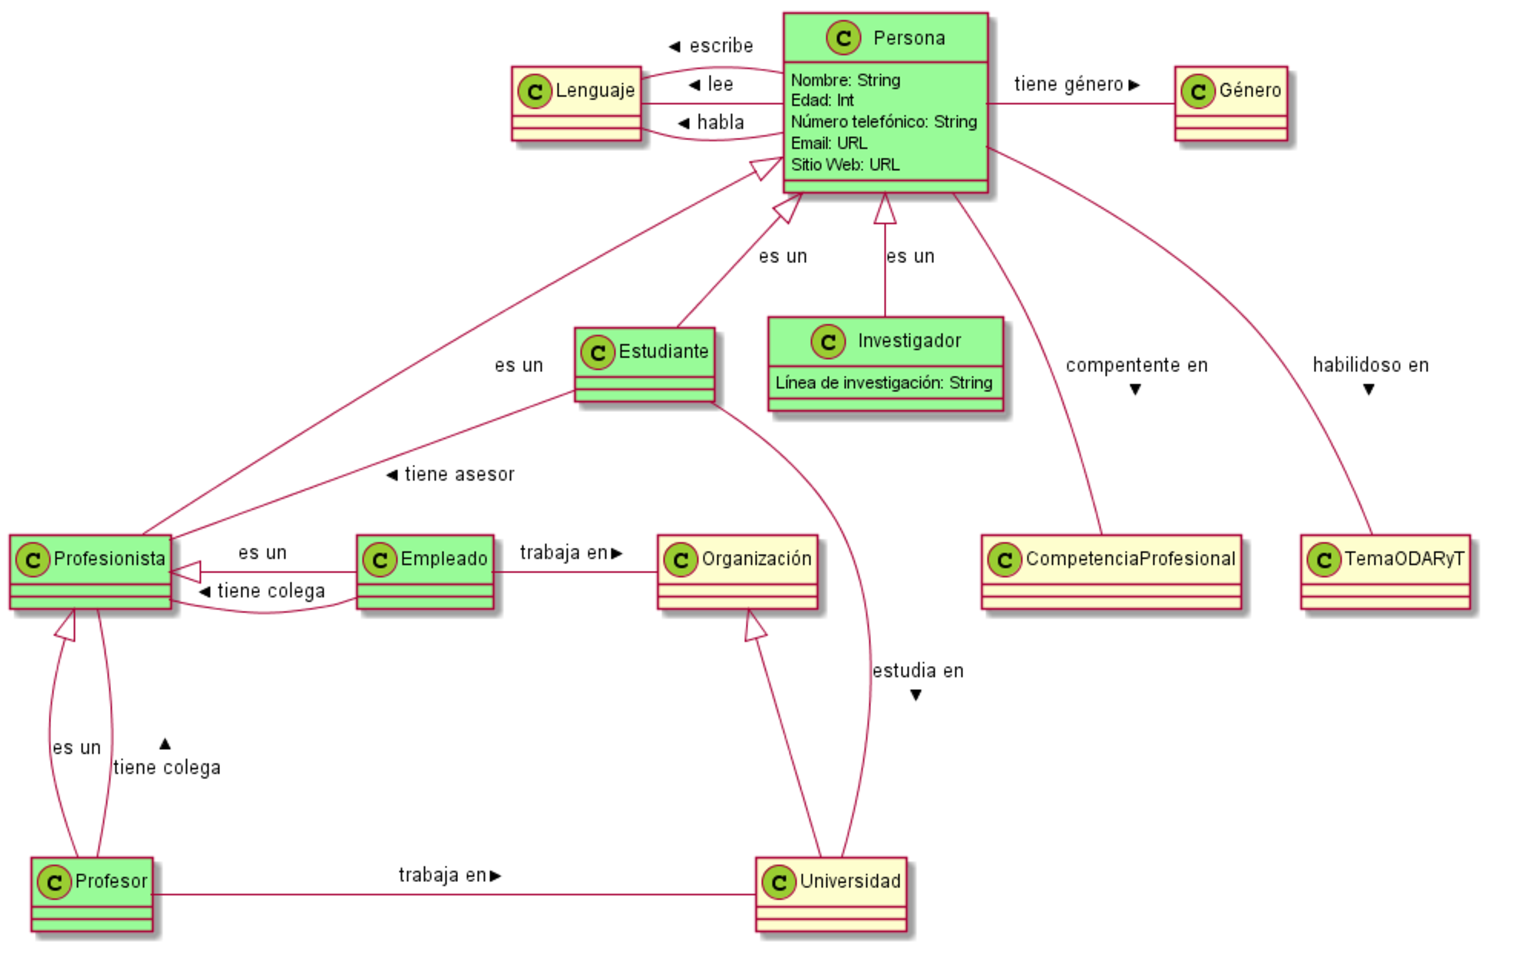
\includegraphics[scale=0.415]{CasoUsoCartComp} 
	\end{figure}
\end{frame}

\subsubsection{Representar el conocimiento e informaci�n mediante el est�ndar RDF}
\begin{frame}[allowframebreaks]
	\frametitle{Representar el conocimiento e informaci�n mediante el est�ndar RDF}
	%%%%%%%%%%%%%%%%%%%%%%%
	\begin{block}{Actividades en la representaci�n del conocimiento}
	\begin{enumerate}
	\item \justifying Asignar un identificador �nico de recursos para cada recurso de informaci�n en la memoria corporativa.
	\item \justifying Asignar los identificadores �nicos de recursos a las propiedades.
	\item \justifying Reconocer los valores de las propiedades: otro recurso o literal.
	\item \justifying Generar las tripletas RDF asociadas a las descripciones de los recursos de informaci�n.
	\end{enumerate}
	\end{block}

	\begin{figure}
	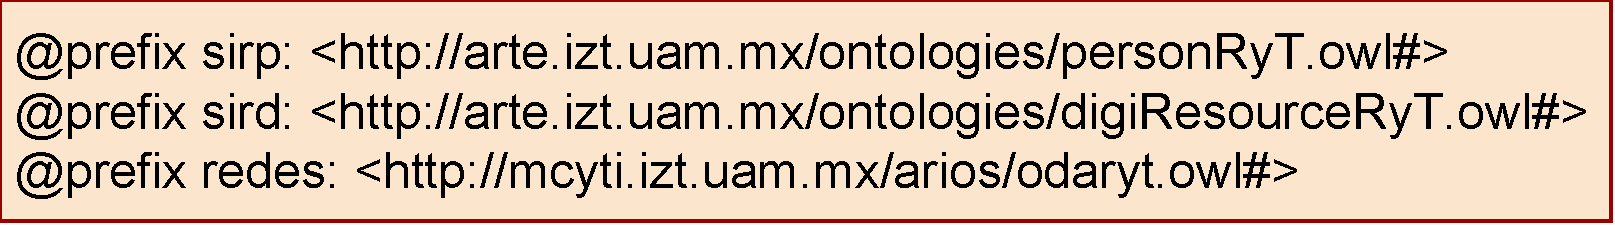
\includegraphics[scale=0.4]{Prefijos} 
	\end{figure}
	%%%%%%%%%%%%%%%%%%%%%%%
	
	\begin{figure}
	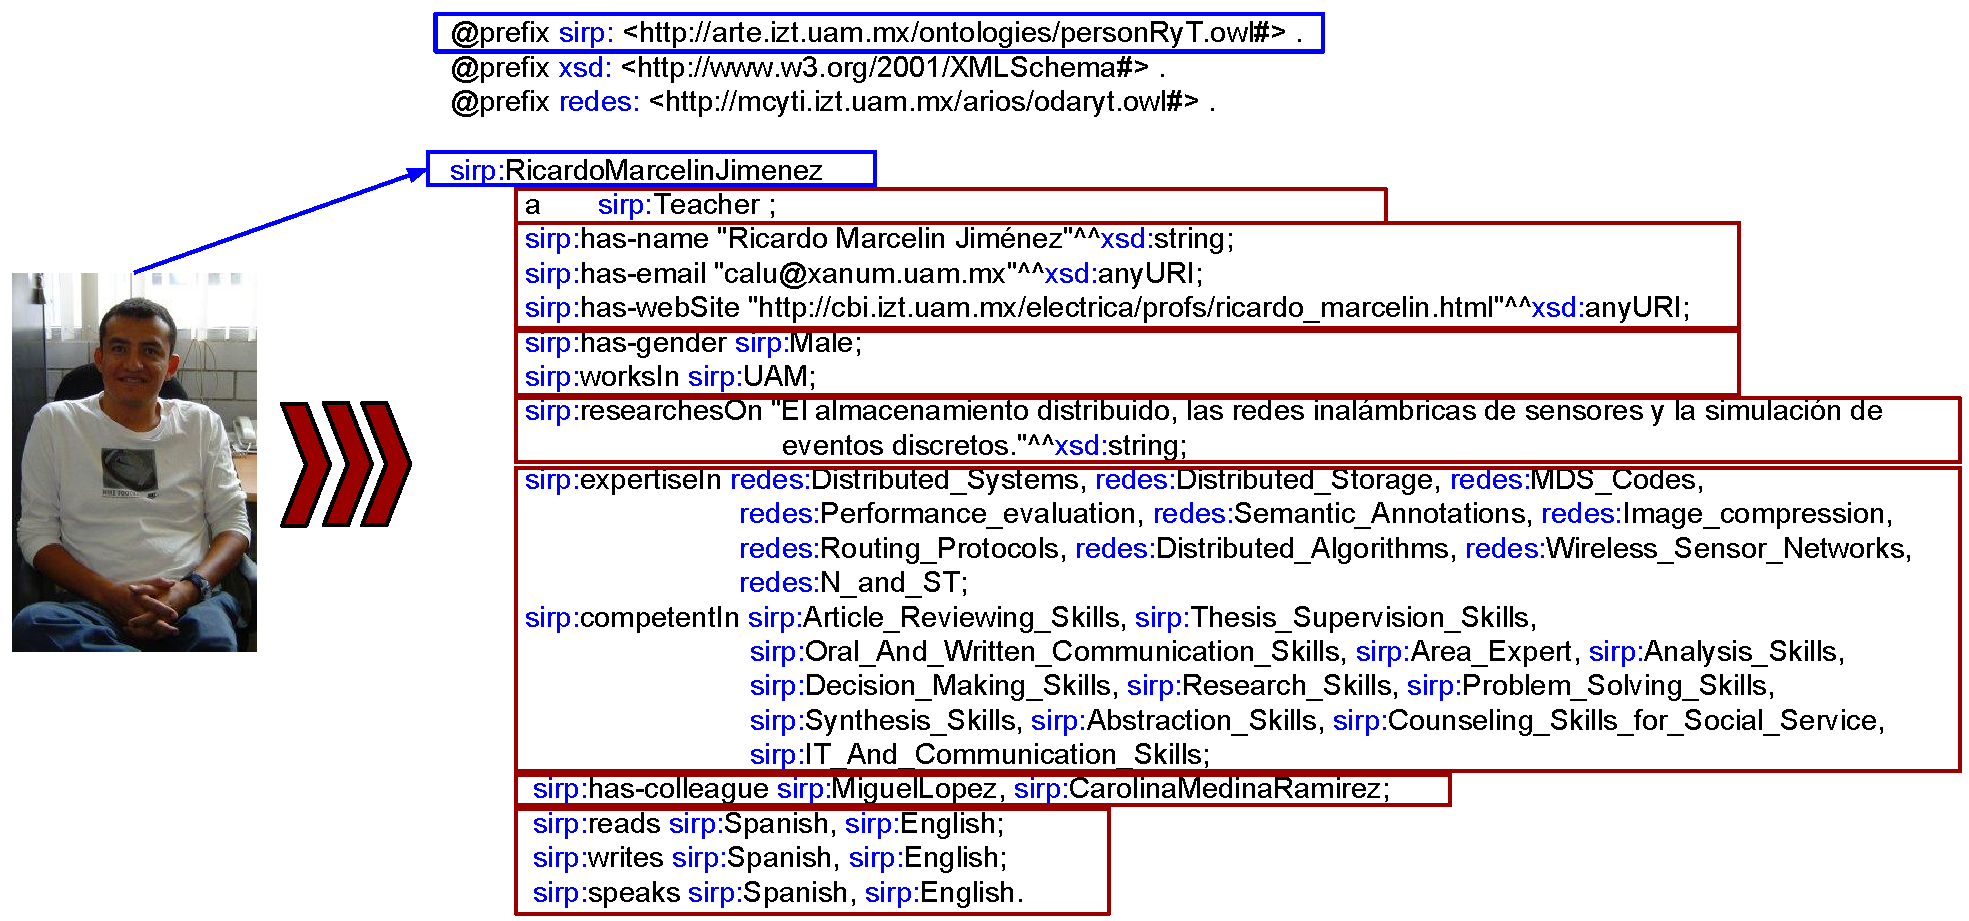
\includegraphics[scale=0.35]{Person2RDF}
	%\caption{Ejemplo de declaraciones del Dr. Ricardo Marcelin Jim�nez en forma de tripletas RDF}
	\end{figure}
	%%%%%%%%%%%%%%%%%%%%%%%
	
	\begin{figure}
	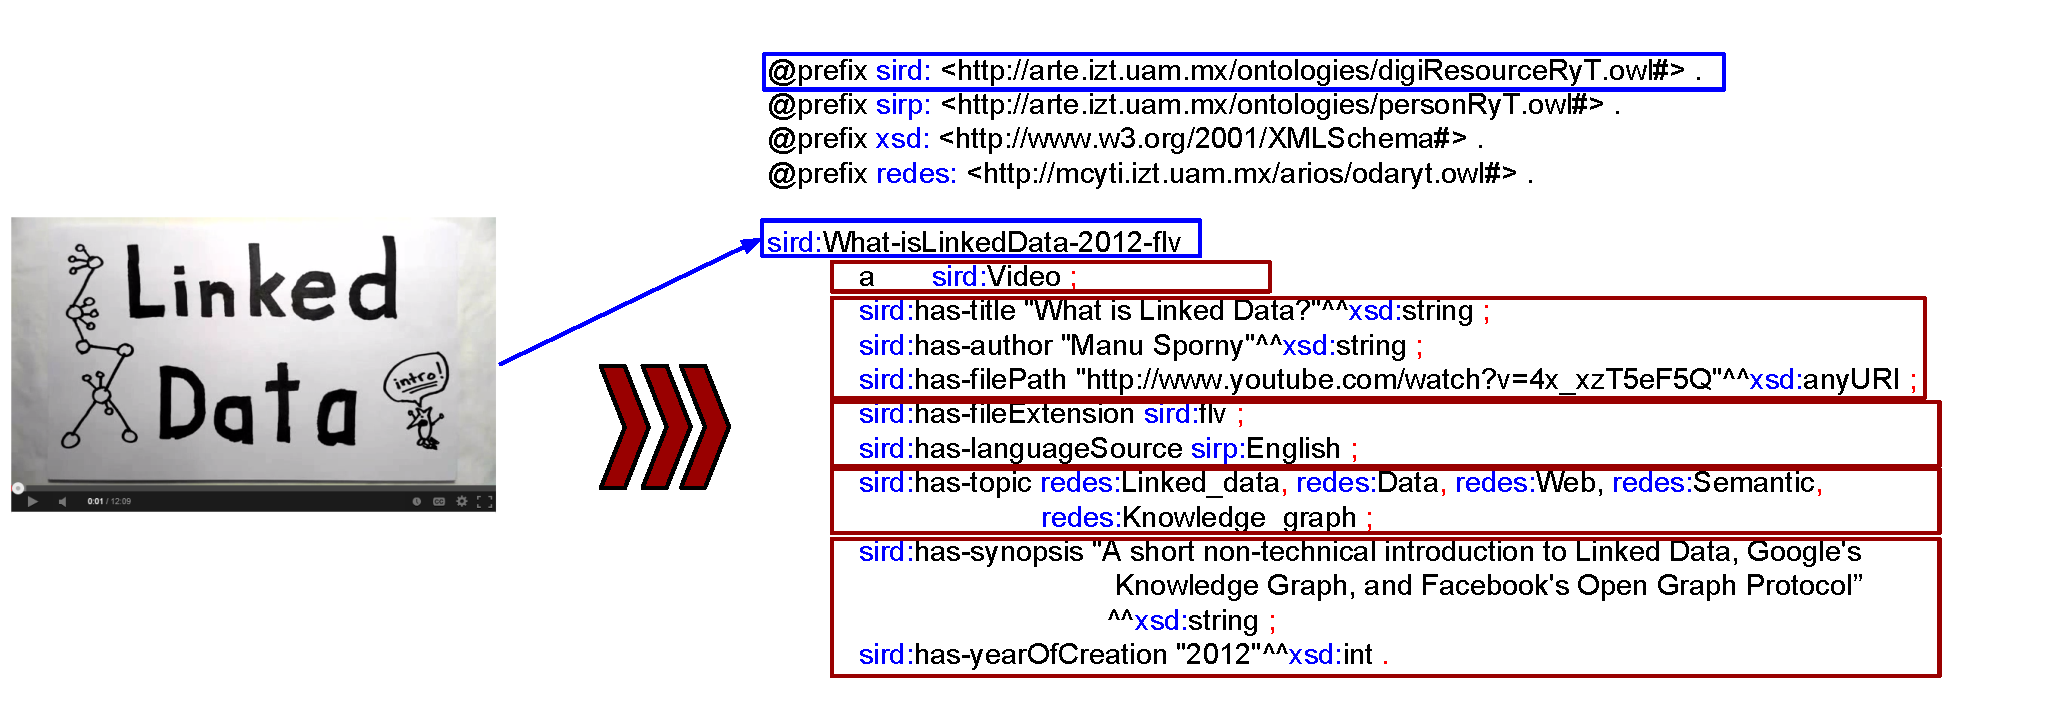
\includegraphics[scale=0.35]{Vid2RDF}
	%\caption{Ejemplo de declaraciones del v�deo ``What is Linked Data?'' en forma de tripletas RDF}
	\end{figure}
	%%%%%%%%%%%%%%%%%%%%%%%
	
\end{frame} 
%%%%%%%%%%%%%%%%%%%%%%%%%%%%%%%%%%%%%%%%%%%%%%%%%%%%%%%%%%%%%%%%%%%%%%%%%%%%%%